\chapter{Odor discrimination task in mice}
\label{chap:MaxData}
\section{Introduction}
Neuronal models of reinforcement learning assume interactions of midbrain dopaminergic neurons and striatum to compute the differences between anticipated and received outcomes. The nature of this cross-areal interaction is however not fully understood. On this purpose we present an application of the cell-assembly algorithm, at level of pairs, on electrophysiological data from mice.
Dual side in-vivo recordings of electophysiological activity from Ventral Striatum, including Pallidum, (VS) and Ventral Tegmental Area (VTA), allowed us to study directionality between the two regions.
The novel statistical approach presented treats the temporal scale and precision of coherent activity patterns as free parameters, to be determined from the data, thus, instead to make assumption, we deduced from data temporal scales and precision involved in assemblies pairs with units either from both regions or from only one of the two regions, shedding light on VS-VTA interaction temporal structure and VS-VTA directionality.
We can use the term directionality in our case because we use the algorithm at level of inter-regional pairs. It is important to recall that the cell-assembly algorithm returns lags between the units activation in assembly, thus using the algorithm at level of inter-regional pairs provides us the lag between two units activation, of those two units one is in VS and another in VTA, a lag in activation of such kind of pair, indicates which region is preceding the other in activation.
Our nomenclature was such that a positive lag means that VS is prior in activation, a negative lag, vice-versa, means that VTA is preceding the activation of VS.
Taking advantage of well defined neuron typologies classifications both in VS and VTA, we further investigated the specific cell-type composition of the assemblies exhibiting directionality. 
%According to their response properties, neurons in VTA are classified in Type I (dopaminergic), Type II(GABAergic) and Type III; according to their electrophysiological properties, neurons in VS are di-vided in medium spiny neurons (MSN), cholinergic interneurons (CIN), and fast spiking interneurons(FSI), the latter are mostly pallidal units.
\section{Description of experiment and data set}
The task presented is a go/no-go reversal odor discrimination task. Two odors were presented to the mouse, one rewarded (CS+) with reward probability 0.9, the second one unrewarded (CS-). Learning the task consisted in licking at least twice when CS+ was presented (hit trials) and not licking during or after the CS- presentation (correct rejection trials). Once the performance criterion was reached, the contingencies were switched. Lick window was open for an interval ranging from 1500 $ms$ to 2000 $ms$ for different sessions after a delay from 500 $ms$ to 1500 $ms$. Only licks happening in the lick window interval were counted as valid to get the reward.
\begin{figure}
    \centering
    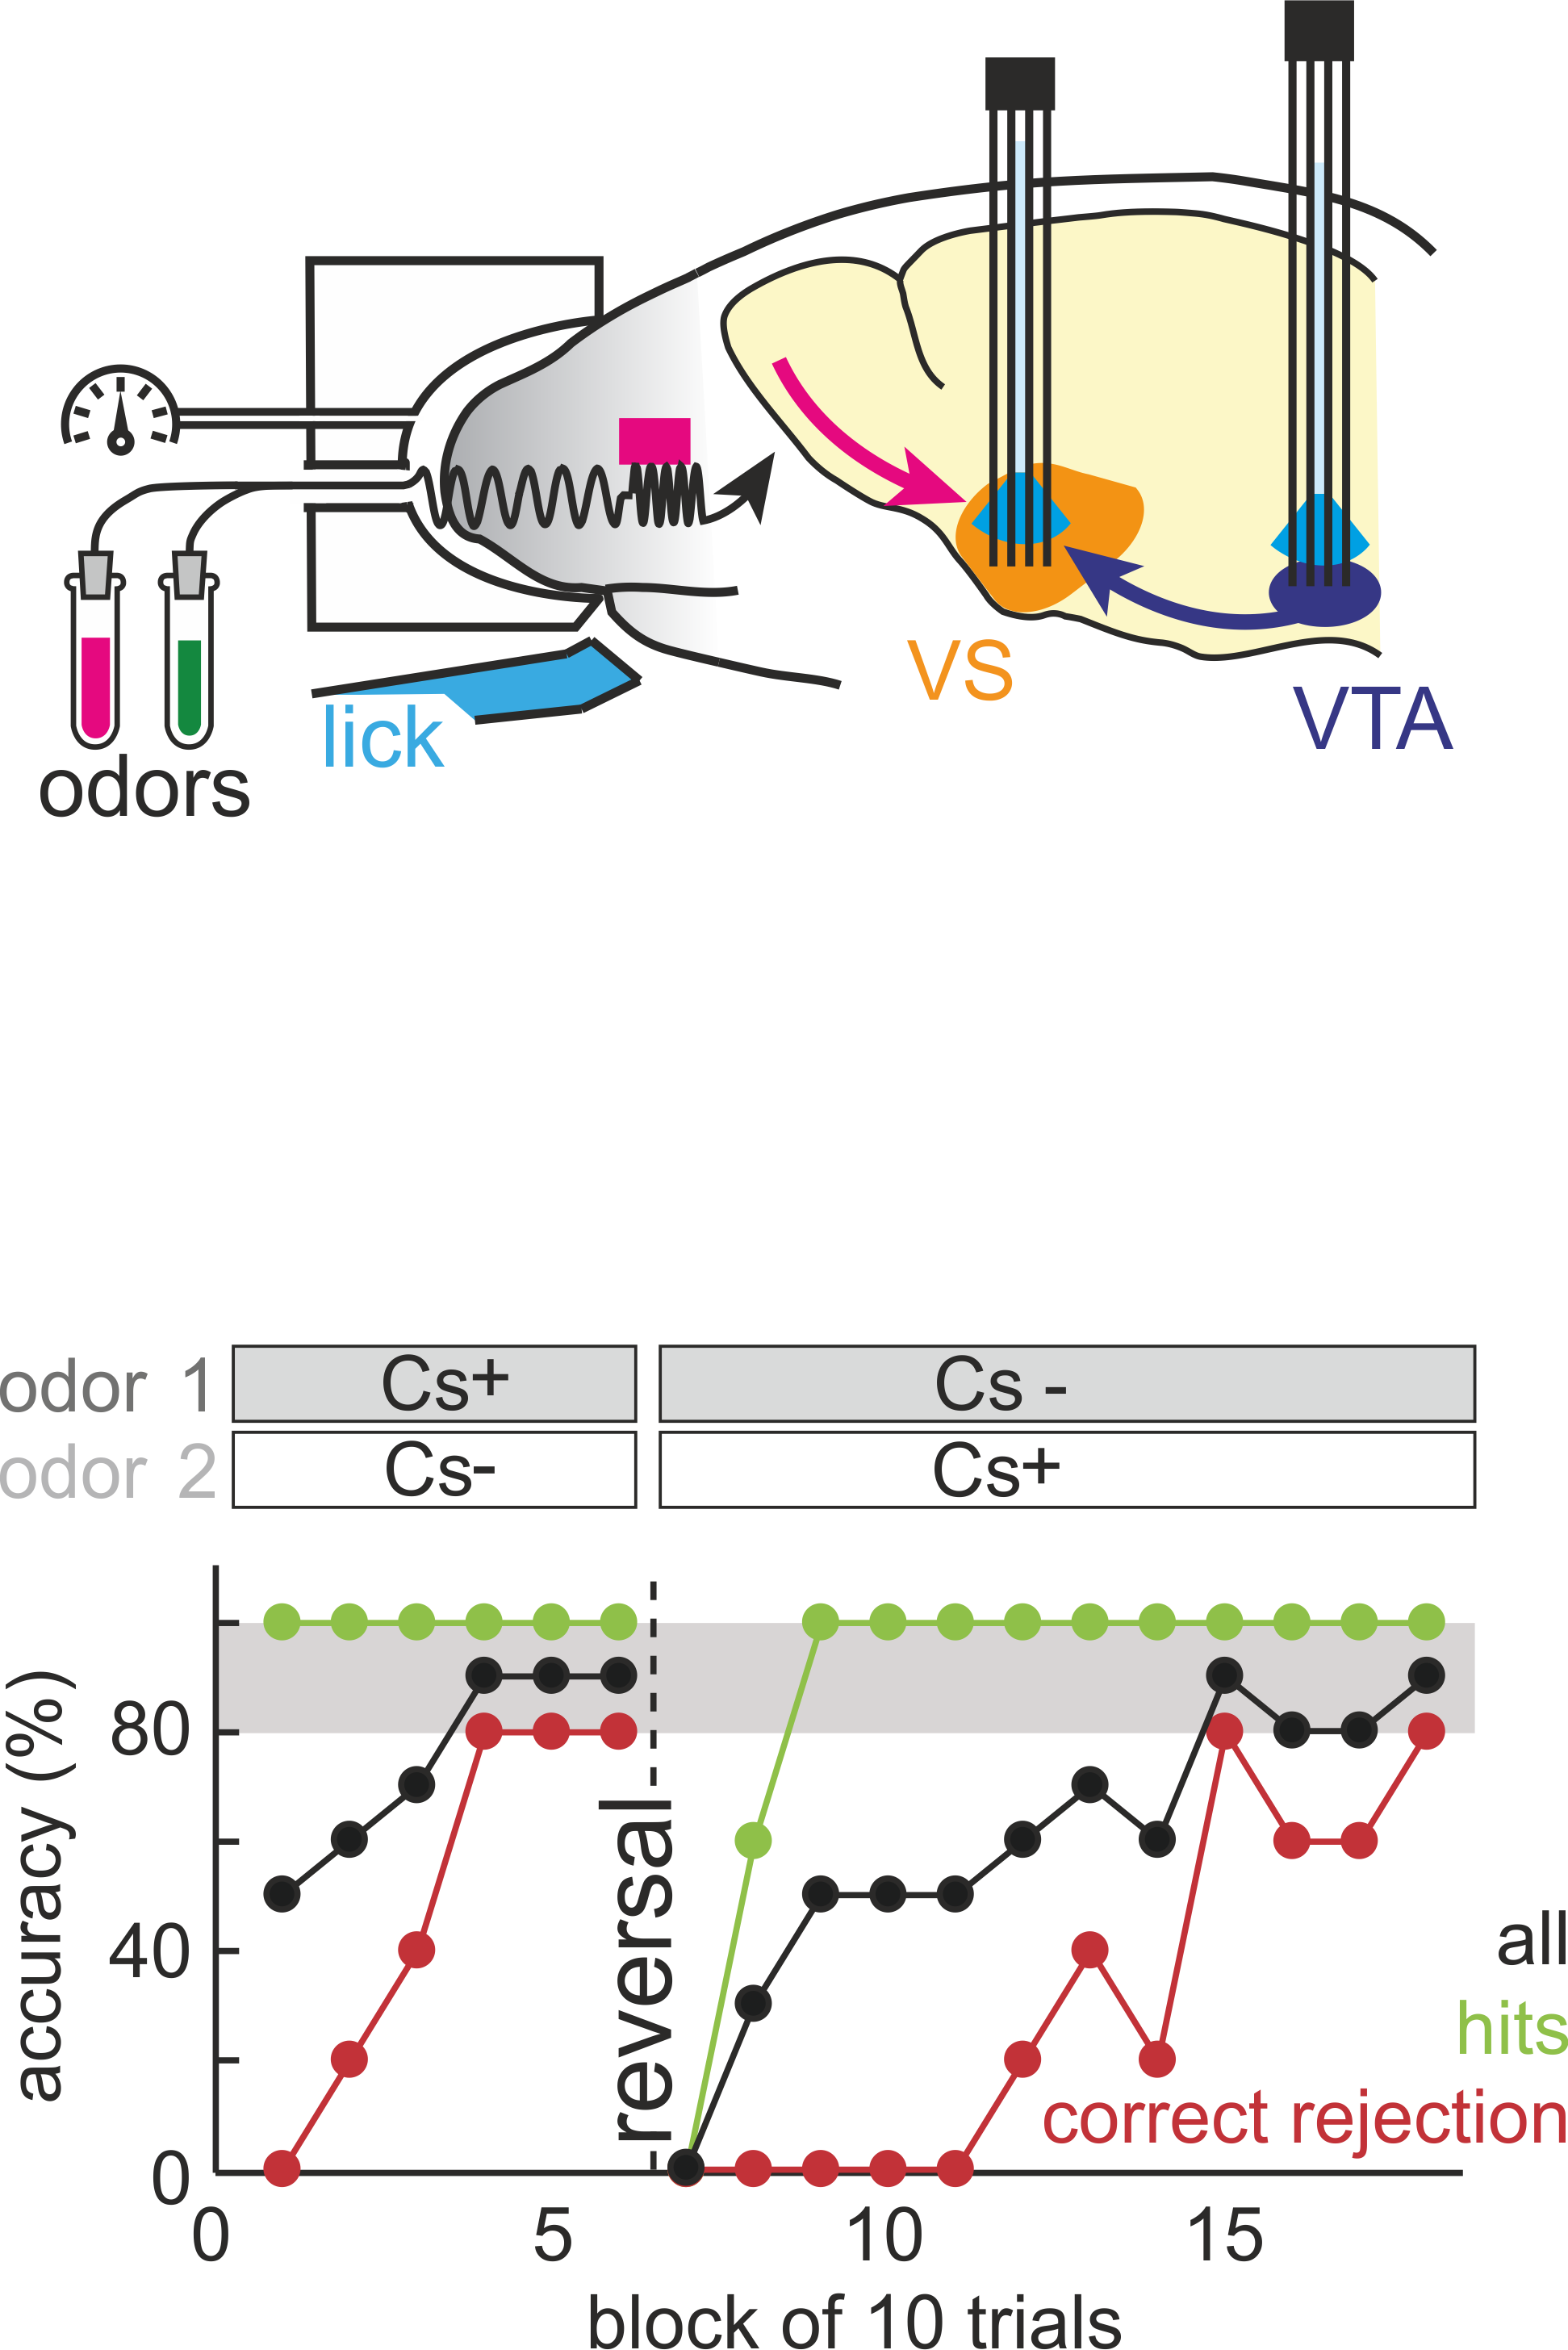
\includegraphics[scale=0.3]{figures/experiment.png}
    \caption{Experimental setup and mice performance}
    \label{fig:experiment}
\end{figure}
\section{Single cells analysis}
We have $803$ VS units and $272$ VTA units in total, that were classified in sub-typologies, specifically VS units were classified as either medium spiny neurons (MSNs), fast-spiking inter-neurons (FSIs) or cholinergic interneurons(CINs), according to their firing pattern characteristics computed using only spikes during the inter-trials interval and after session. Units with a firing rate higher than $12 Hz$ were assigned as FSIs and all units with a firing rate below $2 Hz$ as MSNs. Units in the remaining range were designed as putative regular-firing CINs if the CV or their $ISI$ distribution was less than $1.2$ and ISIs less than $60 ms$ contributed no more than $20\%$ of all ISIs. Finally the resting units were characterized as MSNs or FSIs if they ever were silent for more than $2 s$. Unsing this classification mean normalized autocorrelations and mean waveforms have canonical patterns ({\color{red}I don't know if I can borrow the figure from Max and whether put the figure here or in the appendix}). %(\ref{fig:AutoVS}).
VTA units were instead classified as Type I (Dopaminergic units), Type II (Gabaergic units), and Type III according to their task related activity using a clustering approach adapted from (\cite{Uchida}). First, response were characterized for the relevant time spans ({\color{red}ask Max for the updated intervals}(CS+ from 0 to 0.5 and US from -0.5 to 0 and from 0 to 0.5), significant task related response were assessed with Friedman test, and only significant units ($p<0.05$) were included in the clustering classification.{\color{red}part of classification has to be included}
%\begin{figure}
 %   \centering
  %  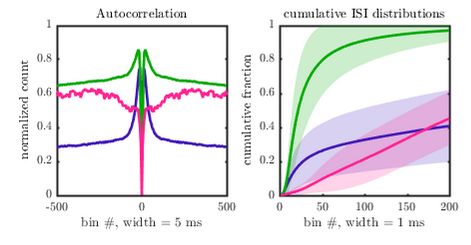
\includegraphics[scale=0.7]{figures/AutocorrelationVSunits.png}
   % \caption{Caption}
    %\label{fig:AutoVS}
%\end{figure}({\color{red}citation of graybiel 2005 if it is the rigth paper})
%distributed as shown in fig.(\ref{fig:GlobalPie})
\section{Preliminary cell assemblies results}
\begin{figure}
    \centering
    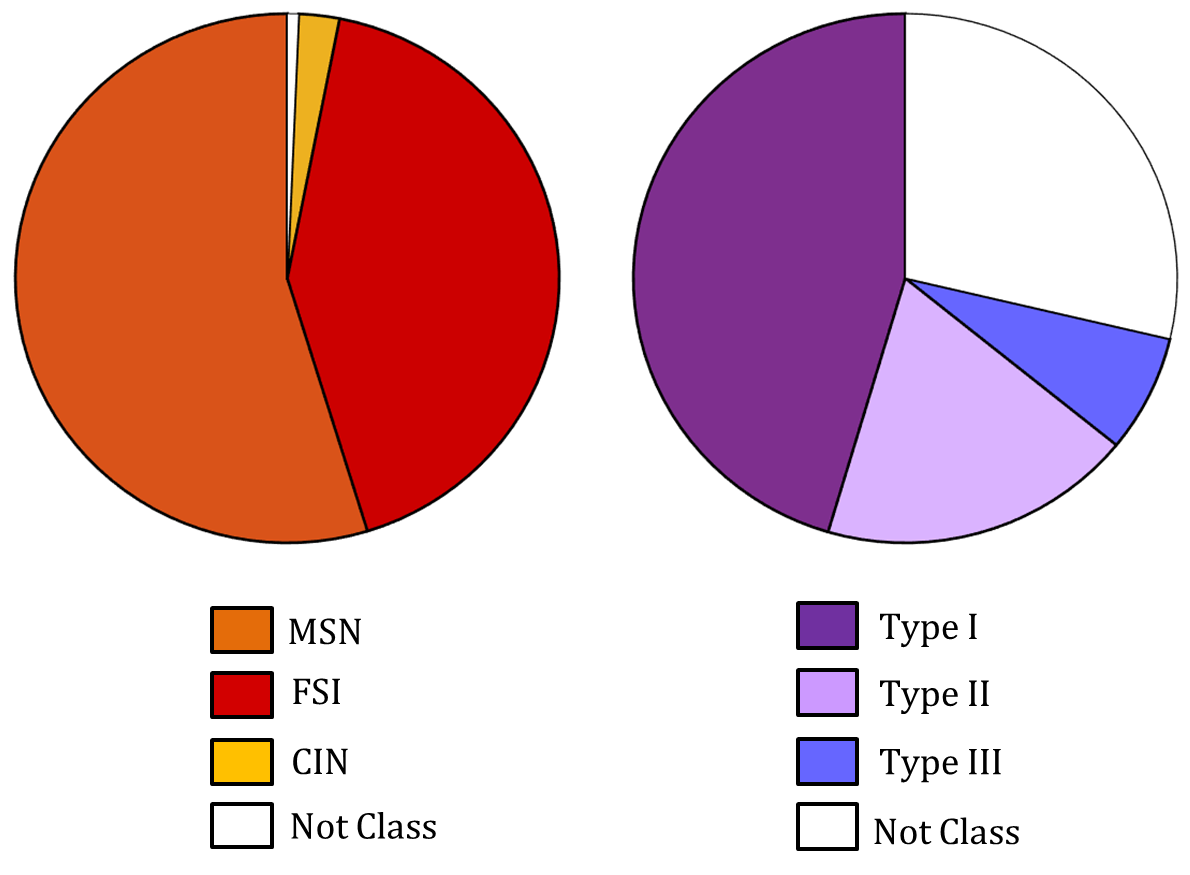
\includegraphics[scale=0.3]{figures/GlobalRegionPieandLegenda1.png}
    \caption{Pie charts of neuron typologies in VS and VTA }
    \label{fig:GlobalPie}
\end{figure}
Preliminary cell assemblies analysis were aimed to understand the size of the concentration of the shared pairs, namely how many units are involved in pairs and, among those, how the units typologies were distributed in assembly pairs. Classified units were distributed in the two regions as shown in fig. (\ref{fig:GlobalPie})

{\color{red} Include figure pie charts for all reversal paradigma}
\section{Time scales, directionality}
Applying the cell-assembly algorithm we were able to detect synchronous ($lag=0$) and asynchronous ($lag\neq 0$) cell assemblies at arbitrary time scale ($\Delta$). Time scales distribution results to be different for intra- regional assembly pairs (pairs with units from VS or VTA) and inter-regional assemblies pairs (pairs with units from both VS and VTA). It's important to point out that, in case of inter-regional pairs, the lag distribution it's a instruments to measure directionality between two regions, indicating which unit fires first leading the activation pattern activity and which one consequently follows. In our case $lag >0$ means VS precedes in activity VTA, and $lag <0$ the opposite, $lag=0$ means that the two units are  simultaneous in activation at the precision of the time scale at which are detected.
We start our analysis from time scales distribution involved in detection pairs.
\begin{figure}[H]
\centering
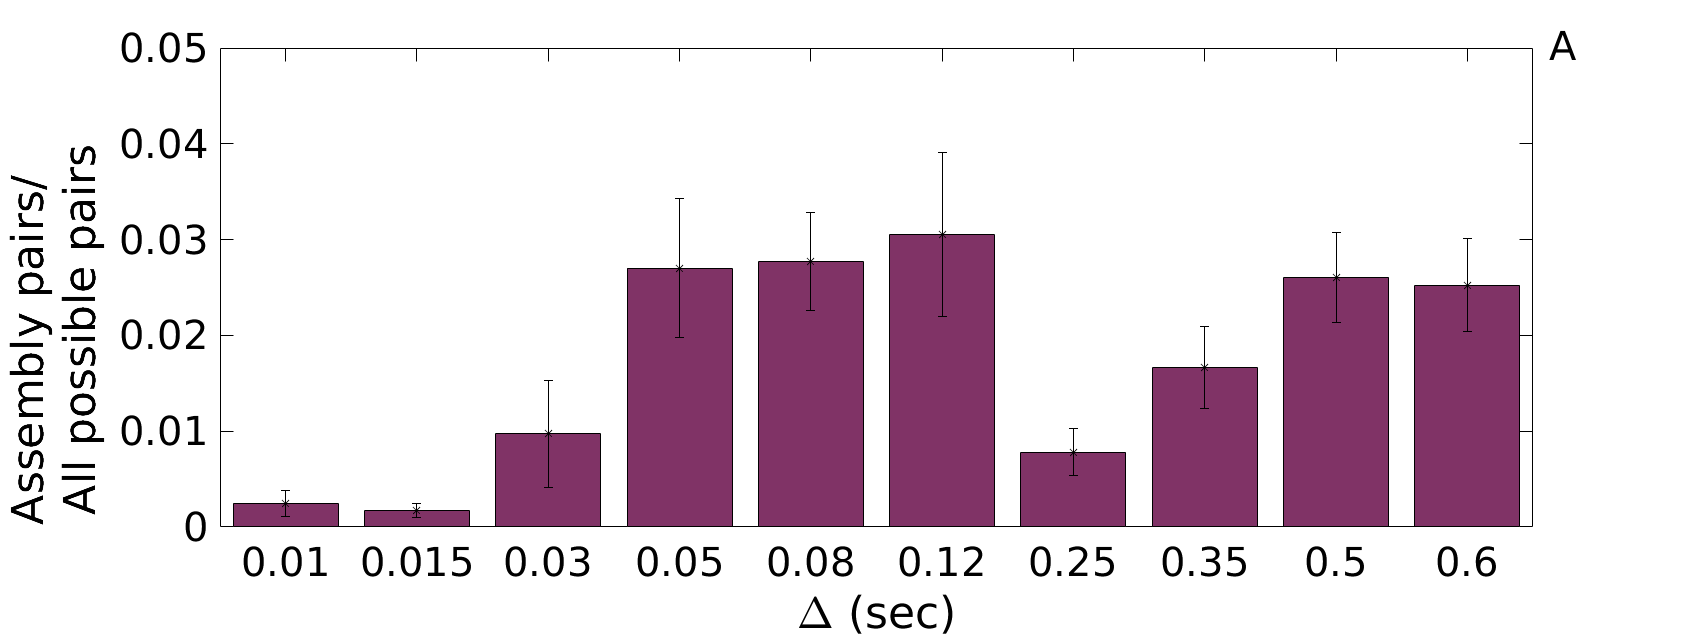
\includegraphics[scale=0.2]{figures/VS_VTA_SLet.png}
%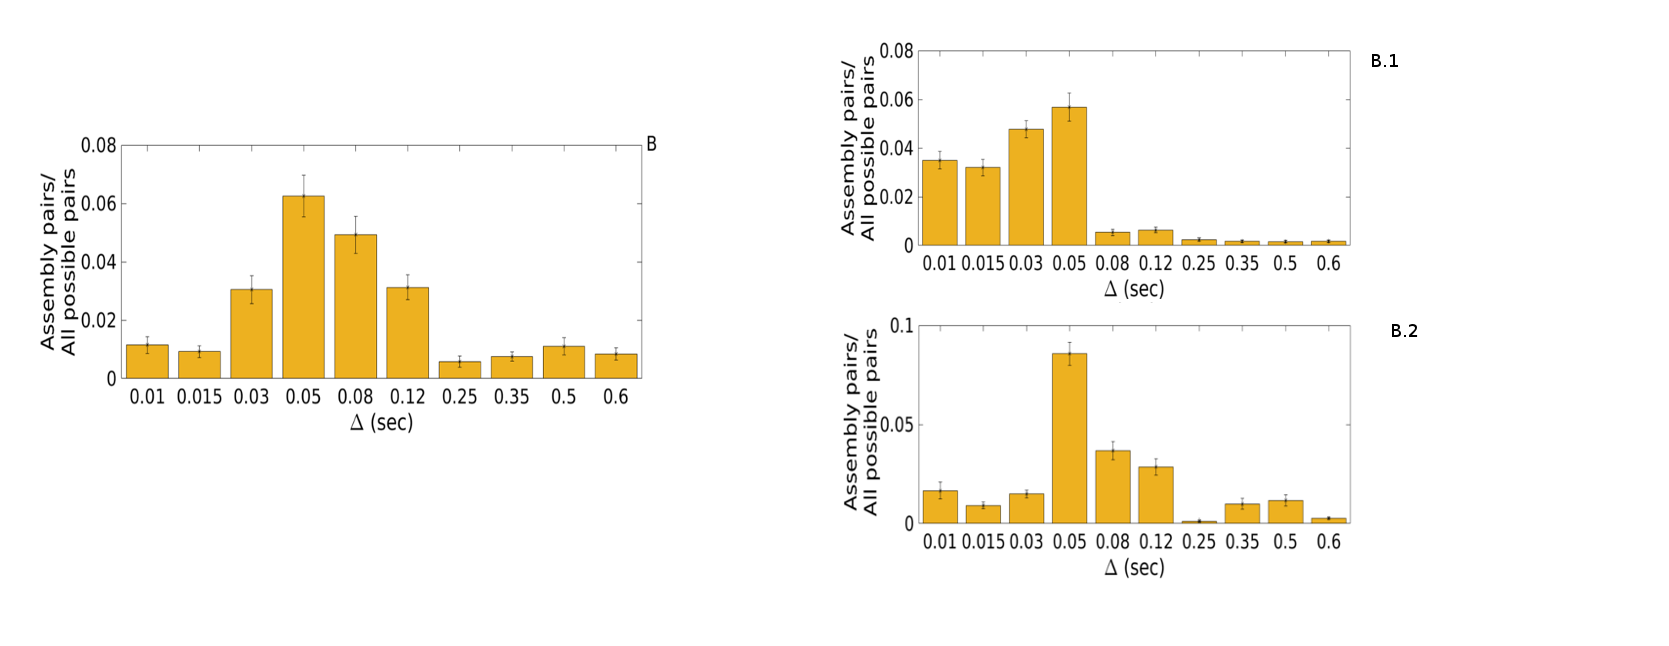
\includegraphics[scale=0.4]{figures/VS_VS_SLet1.png}
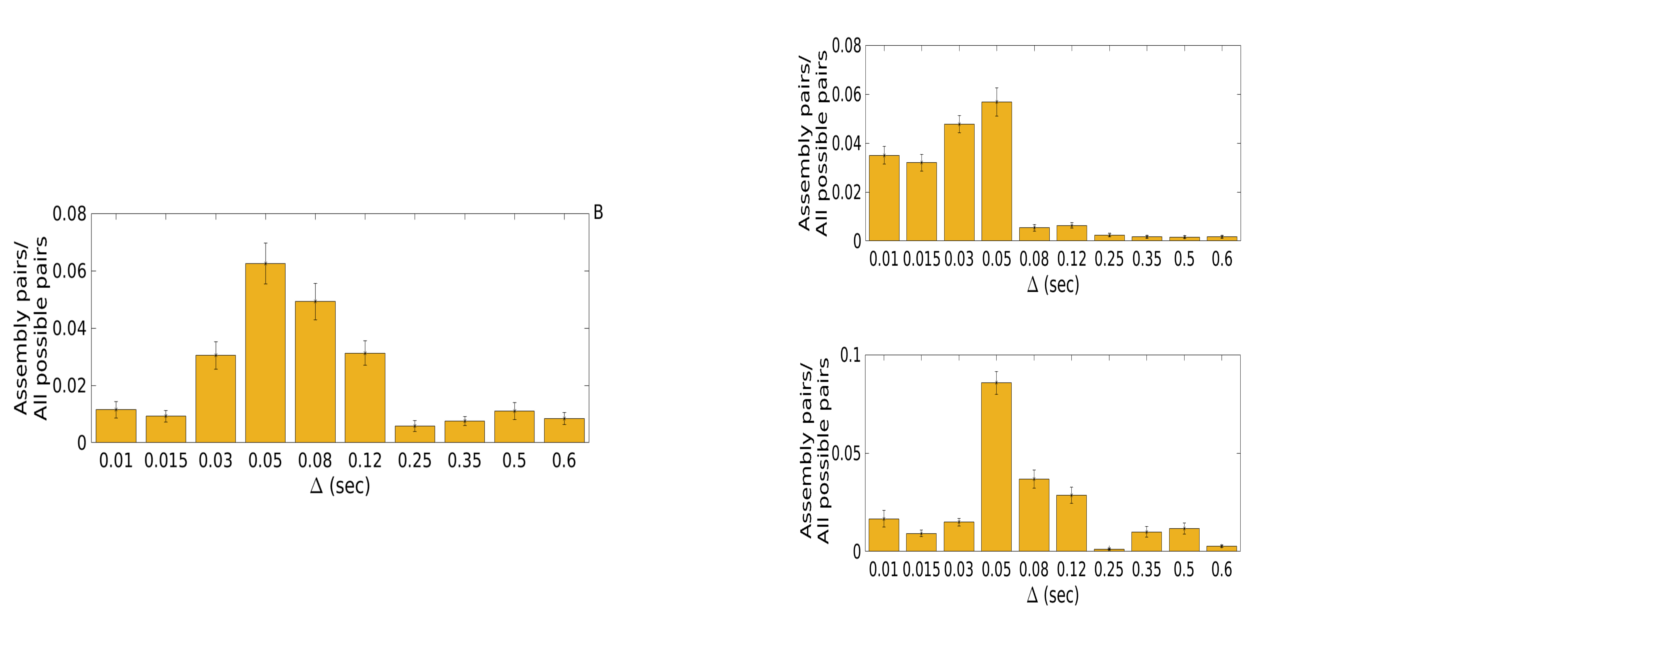
\includegraphics[scale=0.4]{figures/AllBinVSVS.png}
%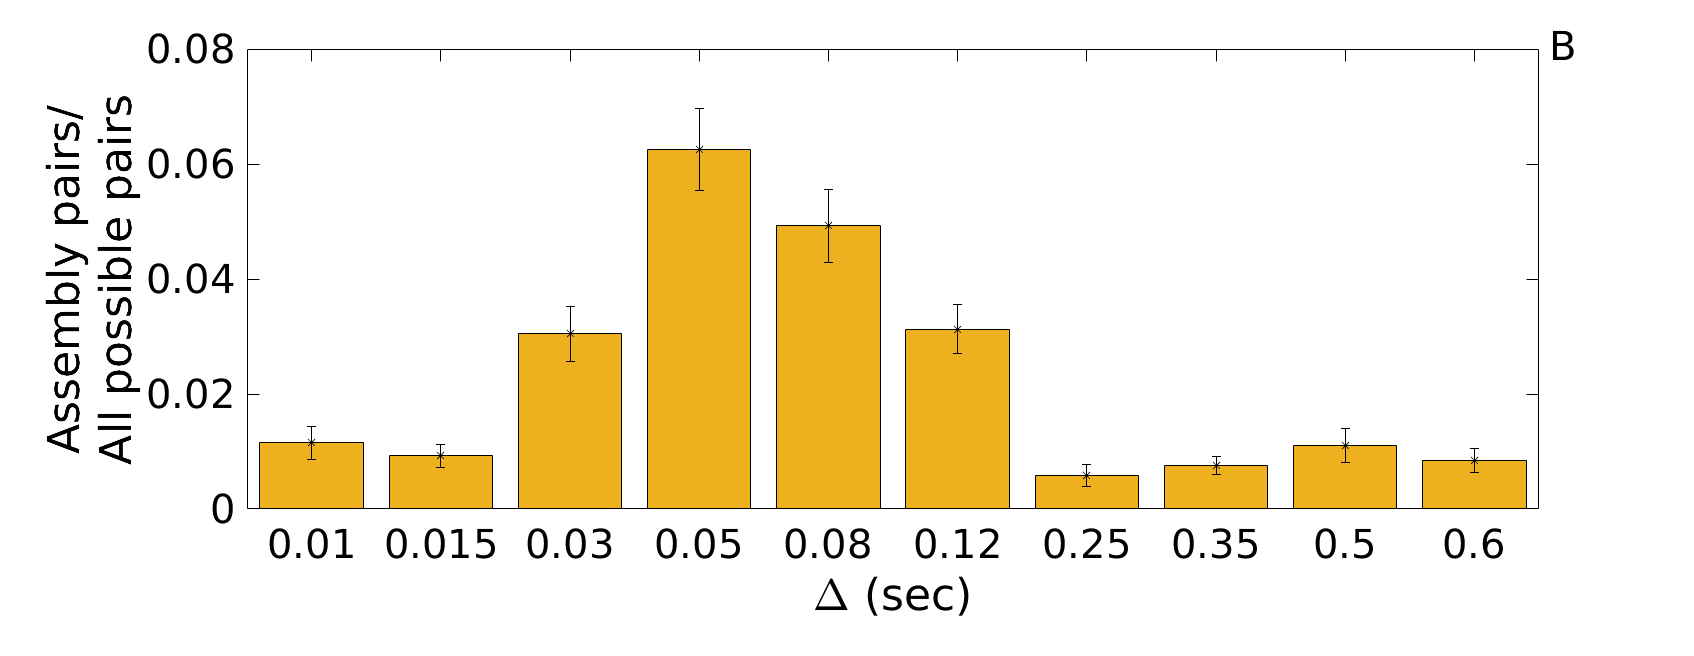
\includegraphics[scale=0.2]{figures/VS_VS_SLet.png}
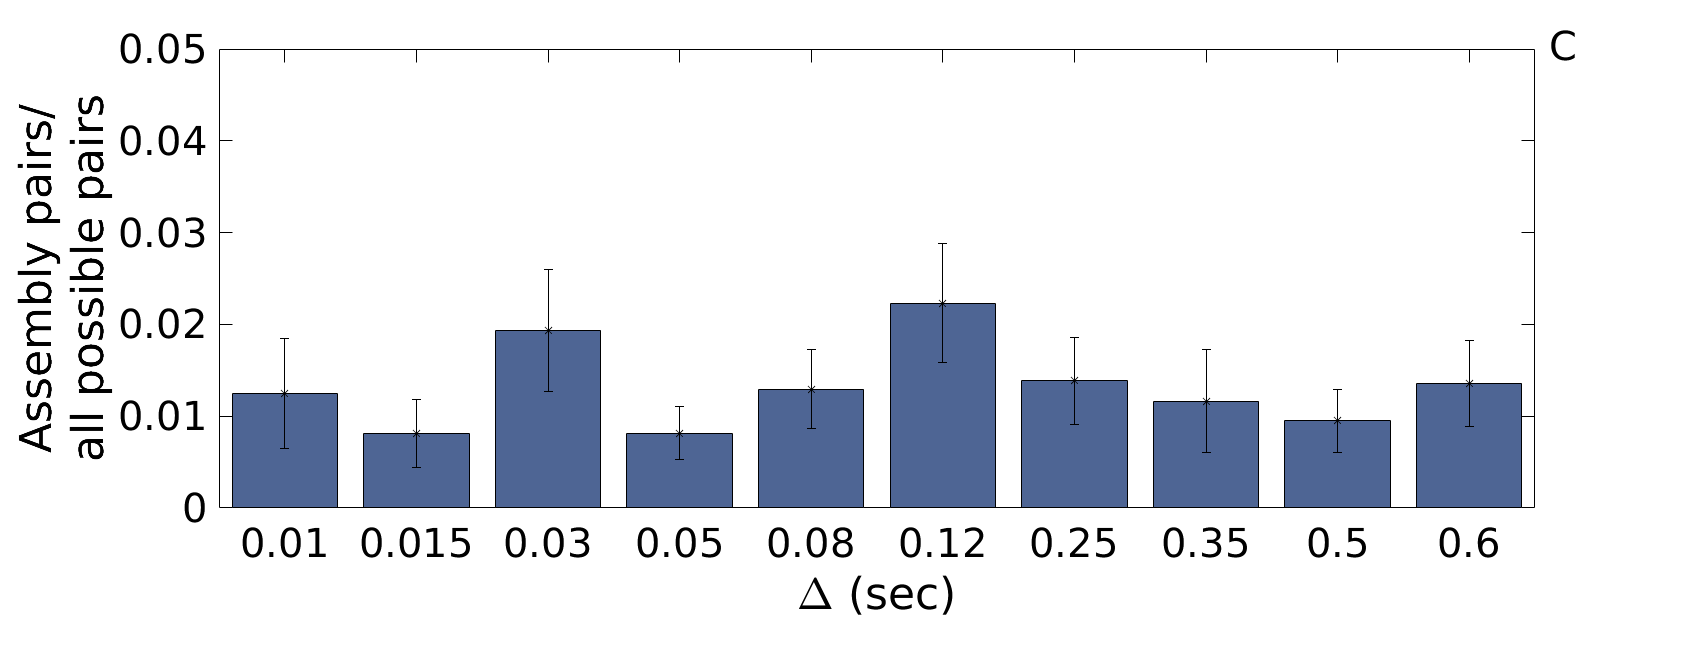
\includegraphics[scale=0.2]{figures/VTA_VTA_SLet.png}

\caption{{\color{red}Important!! Re do the figures with GIMPS include text with title} Bin distribution for intra-regional and inter-regional pairs. A) VS-VTA pairs show a bimodal distribution, meaning two temporal scale involved in inter-regional activtion patterns. B) VS-VS pairs bin distribution presents a peak at 50 $ms$, specifically in this region the pairs MSN-FSI high show an highly peaked distribution, almost centered at the peak of 50 $ms$, plot (B.2), while in MSN-FSI low distribution, albeit the peak is still at 50 $ms$, is evident the predominance of very precise time scales, including bins from 10 $ms$ to 50 $ms$, with respect to the larger time scale plot (B.1).}
\label{fig:BinDistr}
\end{figure}
Clear differences in time scales distribution of pairs detected in VS, VTA and VS-VTA emerge in fig.(\ref{fig:BinDistr}). While we observed assemblies of temporal precision at the scale of few tens of milliseconds only within either VS or VTA, assemblies of lower temporal precision were detected across VS-VTA units. The temporal precision of this last group displayed a bimodal distribution with peaks around $80$ milliseconds and one $1.6$ second, revealing the presence of two time scales, the first, preciser, ranged from 10 $ms$ to 250 $ms$, and the second including broader bin sizes. Intra-regional VTA-VTA pairs instead don't present any peak in time scales distribution. Intra-regional VS-VS bin size distribution is peaked around 50 $ms$. In VS we noticed differences between MSN and high-firing-rate FSI pairs and MSN and low-firing-rate FSI bin size distributions: specifically the firsts show higher temporal precision than the latter. {\color{red}{Include Figure of MSN-FSI and caption of bin size distribution}}.
Bin width and lags analysis reveals time scale segregation, that can reveal in turn different assembly-activation patterns. In fig.(\ref{fig:AsActBinLag}) heat maps of assembly activity show differences in activation patterns among different bin width and lag. In the paradigm in examination animals were well-trained, it was the third time that the same couple of odor were presented with the same stimulus duration length.
\begin{figure}
    \centering
    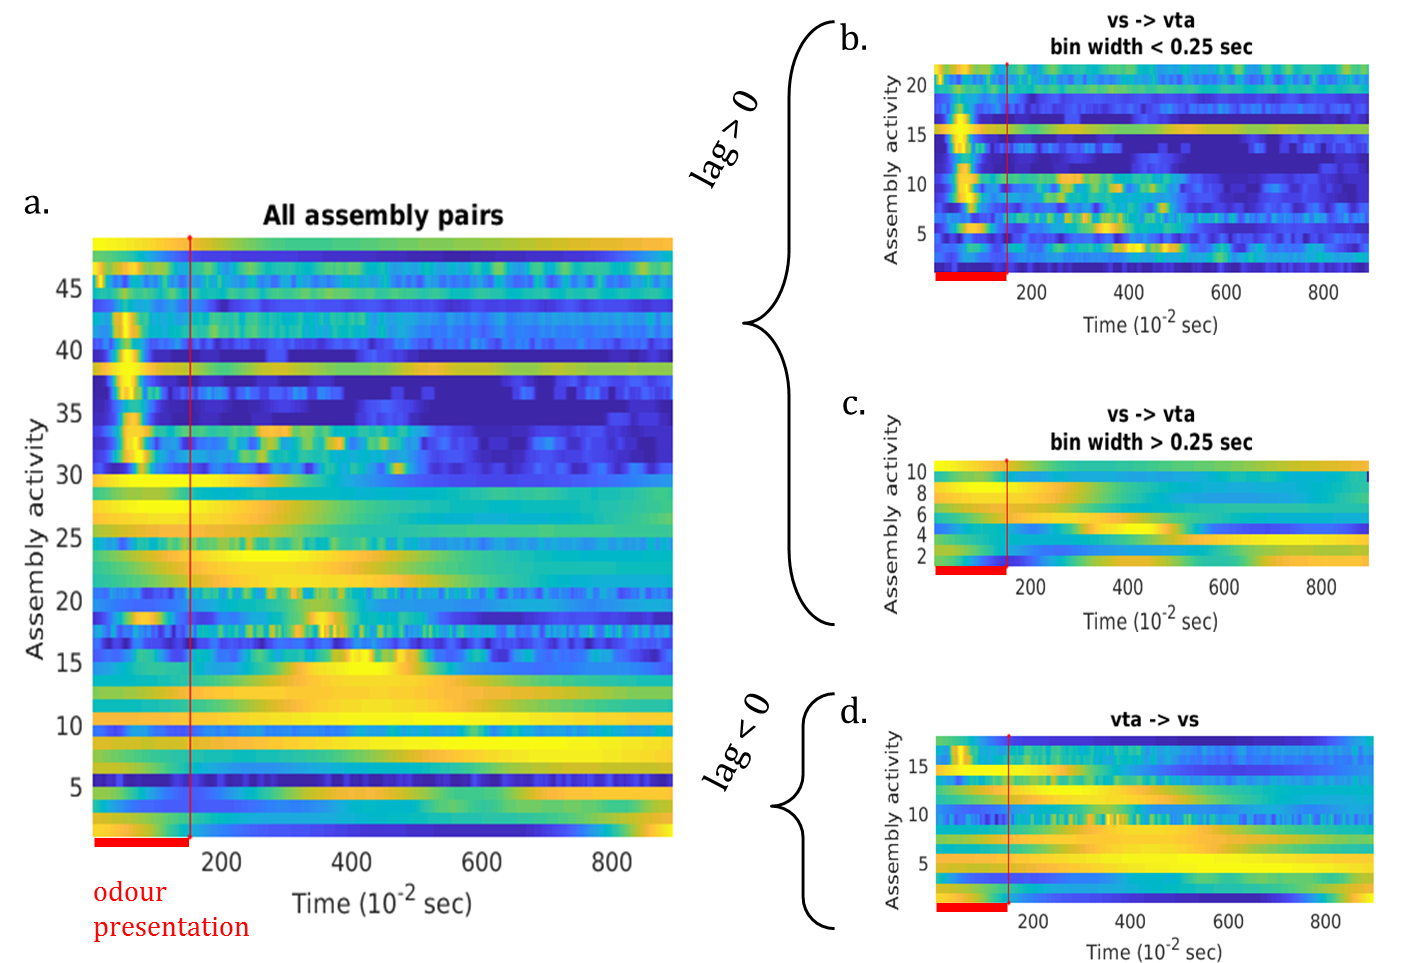
\includegraphics[scale=0.45]{figures/AsActPerBinLag1.png}
    \caption{Assembly-activation patterns given time bins and lags. In a.) totality of assemblies of one experimental paradigm, b,c,d. assemblies of same paradigm of a. selected for bin size ($\Delta$) and lag, $\Delta < 0.25 s$ and $lag > 0$ (b.), $\Delta > 0.25 s$ and $lag > 0$ (c.), $lag < 0$ (d.)}
    \label{fig:AsActBinLag}
\end{figure}
Directionality between VS and VTA was a point of particular interest for our study. The above consideration led us to study separately lag distribution of VS-VTA pairs detected in preciser and broader temporal scales highlighted from bin sizes distribution. 
Interestingly only the lags of more temporally precise assemblies displayed an asymmetric distribution indicating VS leading VTA (fig. \ref{fig:LagInSecAll}). Specifically, these directional assemblies were composed of striatal and pallidal projection neurons leading dopaminergic VTA neurons (MSN and Type I pairs). Importantly, inter unit activation lags of assemblies containing pallidal neurons (FSI) were shorter than those containing striatal projection neurons (MSN), compatibly with assumed connectivity.
\begin{figure}[H]
\centering
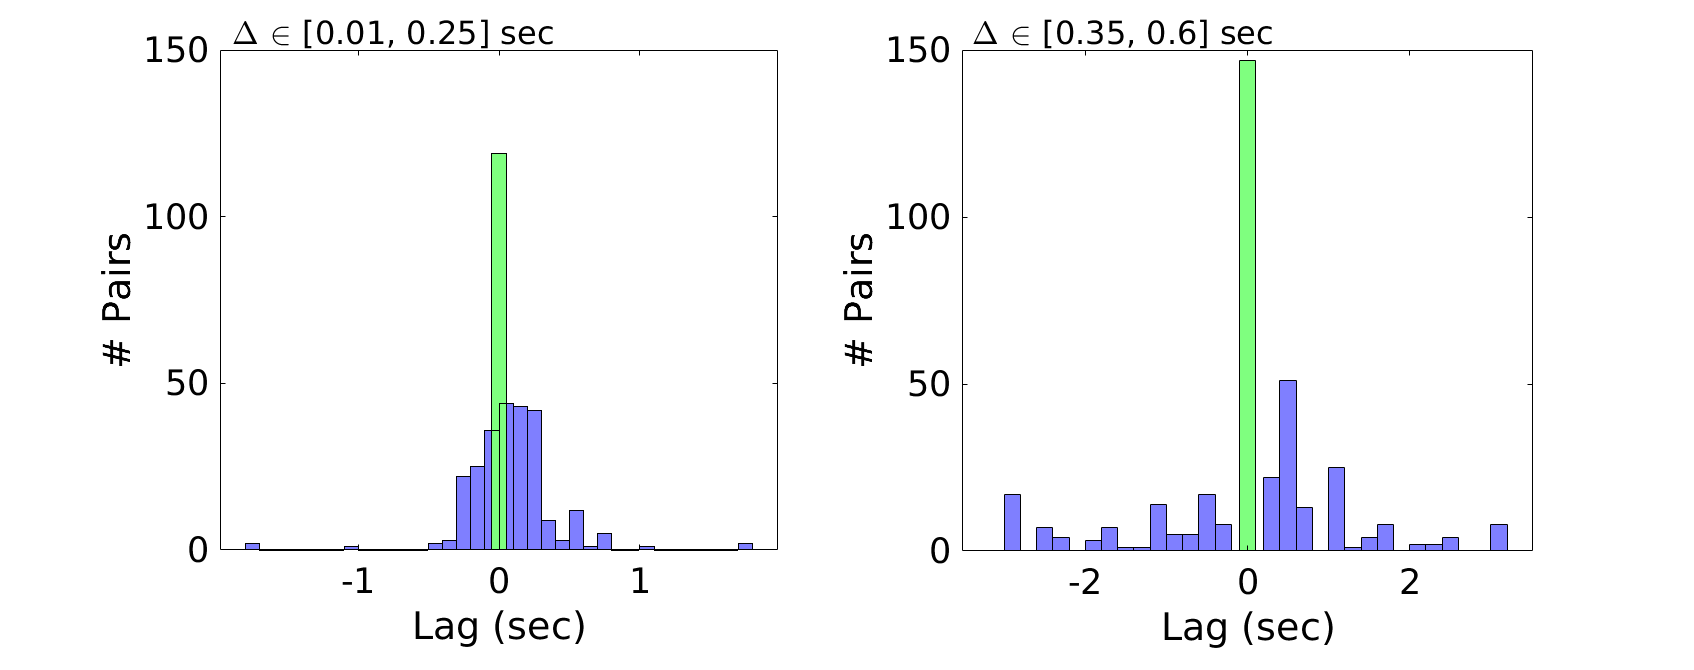
\includegraphics[scale=0.3]{figures/LagGeneralInSec.png}
\caption{Lag distribution for VS-VTA pairs in seconds. In green the synchronous pairs. On the left, lag distribution for pairs detected in preciser time scales. Slight distribution asymmetry indicates directionality in the direction of $lag > 0$, meaning a predominance of pairs in which VS leads VTA. On the right, the lag distribution for pairs detected in the broader time scale.}
\label{fig:LagInSecAll}
\end{figure}

\begin{figure}[H]
\centering
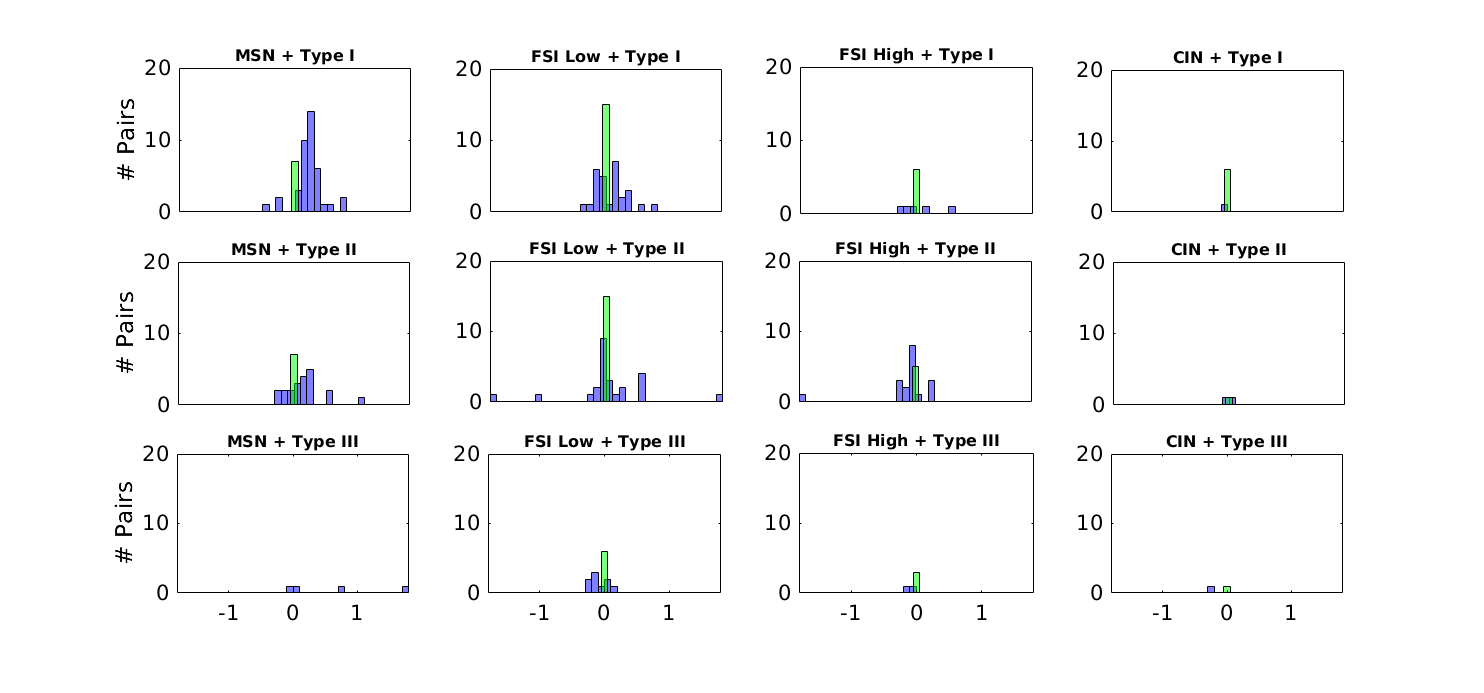
\includegraphics[scale=0.4]{figures/Type_oriz.png}
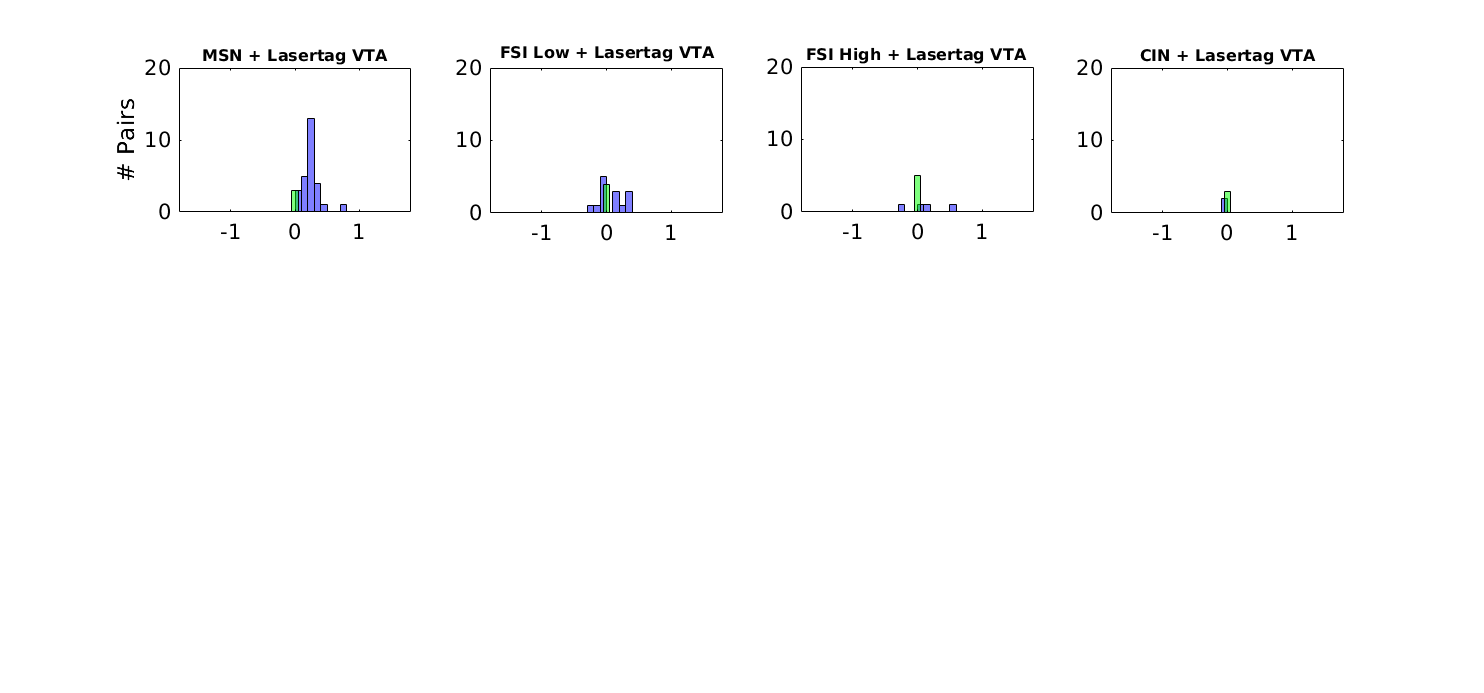
\includegraphics[scale=0.4]{figures/OnlyLaserOriz.png}
\caption{blabla}
\label{fig:LagInSecAll}
\end{figure}
In fig. (\ref{fig:directional_assembly}) a directional assembly. On top is shown mean and standard deviation of the assembly's activity for paired (grey line) and unpaired odor trials (purple line) in the original phase. On bottom raster plot and firing rate (mean and standard deviation) of units in assembly. x-axis origin correspond to the odor onset, while the red line marks the end of the stimulus duration. The examined assembly has a positive lag, that means VS preceding in activity VTA, from neuronal activity we can see in fact the VS unit activate before than the VTA unit. The assembly was detected with a bin size of $0.25 sec$, meaning that we are in the small temporal scale domain, in which the directionality clearly emerged. From the raster plot is evident that this kind of activation was persistent in each trial, in fact that assembly showed a significant task related activity after the stimulus. It is interesting to note the different activation for paired odor trials and unpaired odor trials, revealing the odor discrimination capability of the assembly. 
\begin{figure}
    \centering
    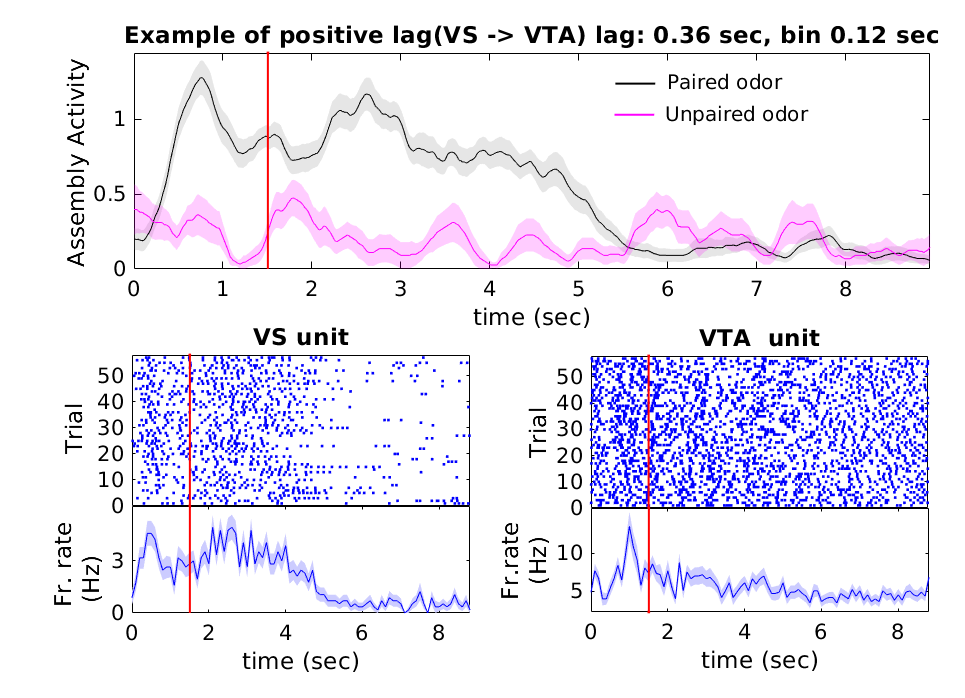
\includegraphics[scale=0.4]{figures/1_21Lastrev1Pru_An4Poster2.png}
    \caption{Directional assembly. On top mean and standard deviation of the assembly's activity for paired (grey) and unpaired odor trials (purple) in the original phase. On bottom raster plot and firing rate (mean and standard deviation) of units in assembly. x-axis origin correspond to the odor onset, while the red line marks the end of the stimulus duration. The examined assembly has a positive lag, that means VS preceding in activity VTA, from neuronal activity we can see in fact the VS unit activate before than the VTA unit.}
    \label{fig:directional_assembly}
\end{figure}
 To better study assemblies activation patterns first the task relevant moments of the experiment were selected, choosing as interval of interest period around the stimulus presentation and the reward delivery, then we analysed the task related assemblies activity in two experimental phases (original and reversal), noting diverse responses among neural typologies involved. For a better visualization of task related activation via heat plots, hit trials (rewarded odor, mouse went for reward), correct rejection trials (unrewarded odor, mouse sat quiet), false alarm trials (unrewarded odor, mouse went for reward), were kept separated, however this separation among trials types was released in further analysis, without affecting results. First difference between original and reversal phase is number of assemblies responding during the post-stimulus interval, this number decrease for all the typologies involved during hit trials (as shown in fig. (\ref{fig:histo_taskrel})), in according to the intuition, in reversal phase in fact, when the animals became more expert, neuronal response tend to be shifted closer to the reward delivery. This effect can be seen in fig. (\ref{fig:NeusInAsse}) where activity and raster plots of two units in a pair are shown. Looking at the raster plots, a shift in correspondence to the phase-switch is evident in both units.
 \begin{figure}
     \centering
     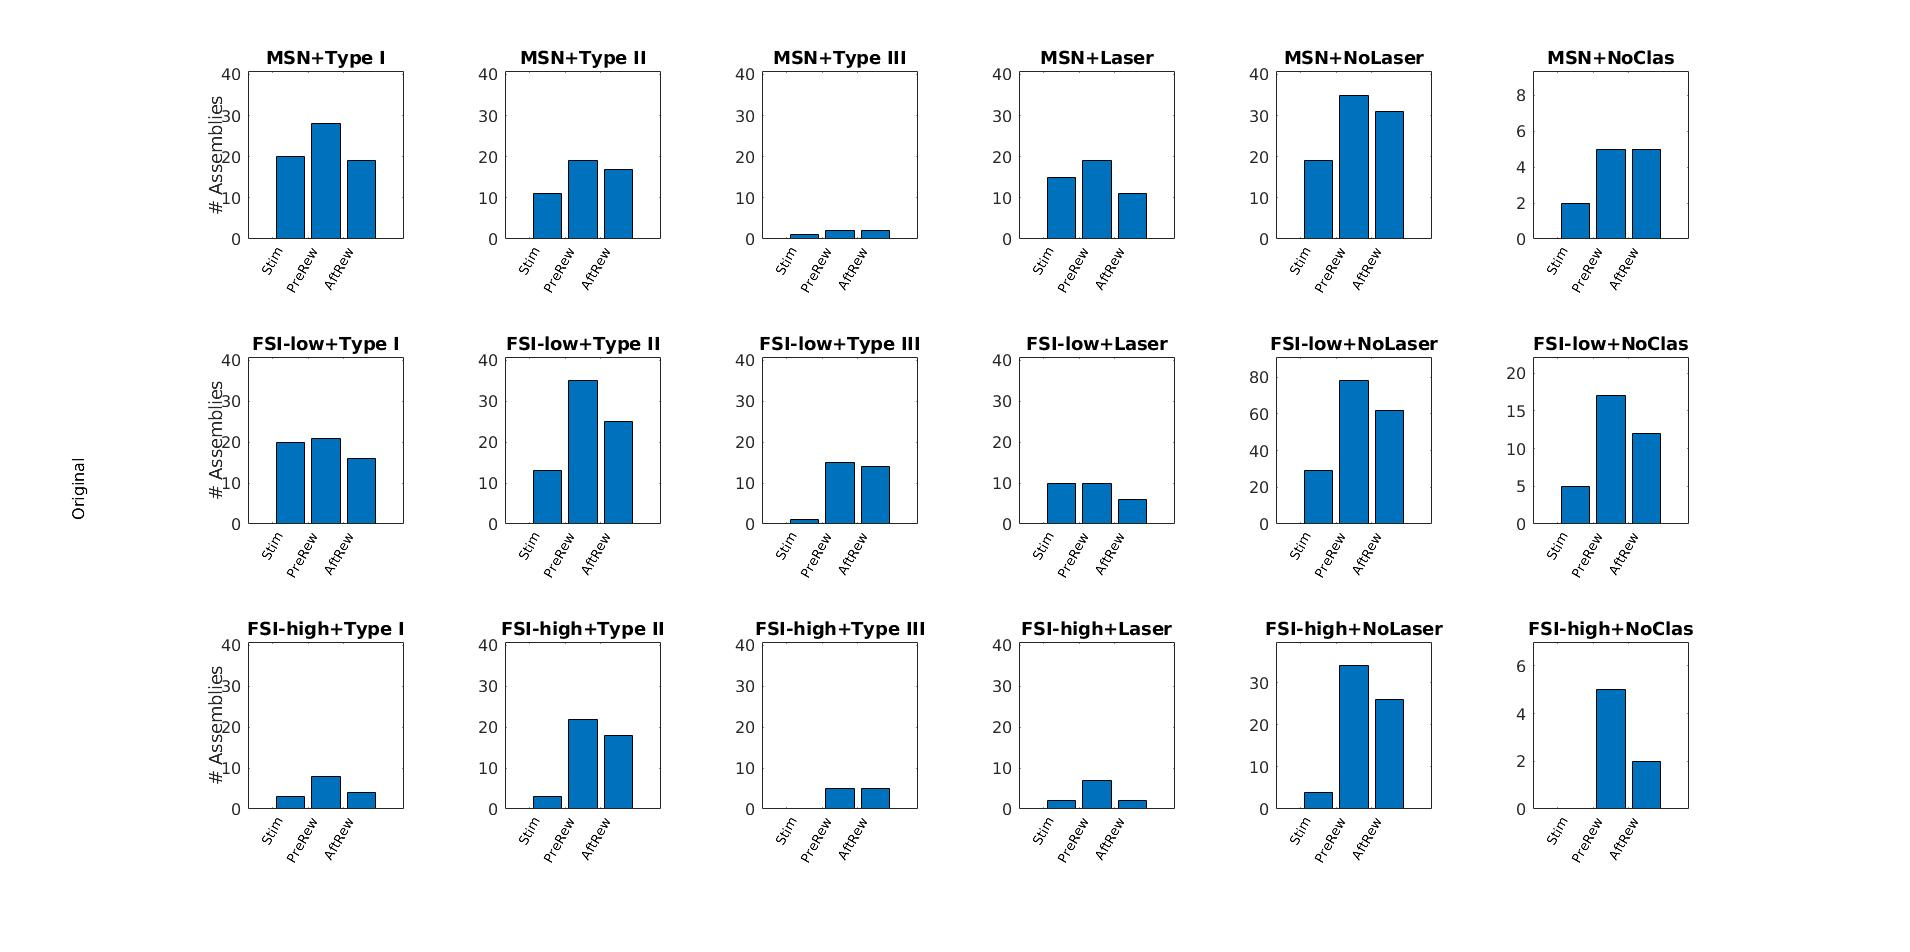
\includegraphics[scale=0.3]{figures/Original_Hit_N.jpg}
     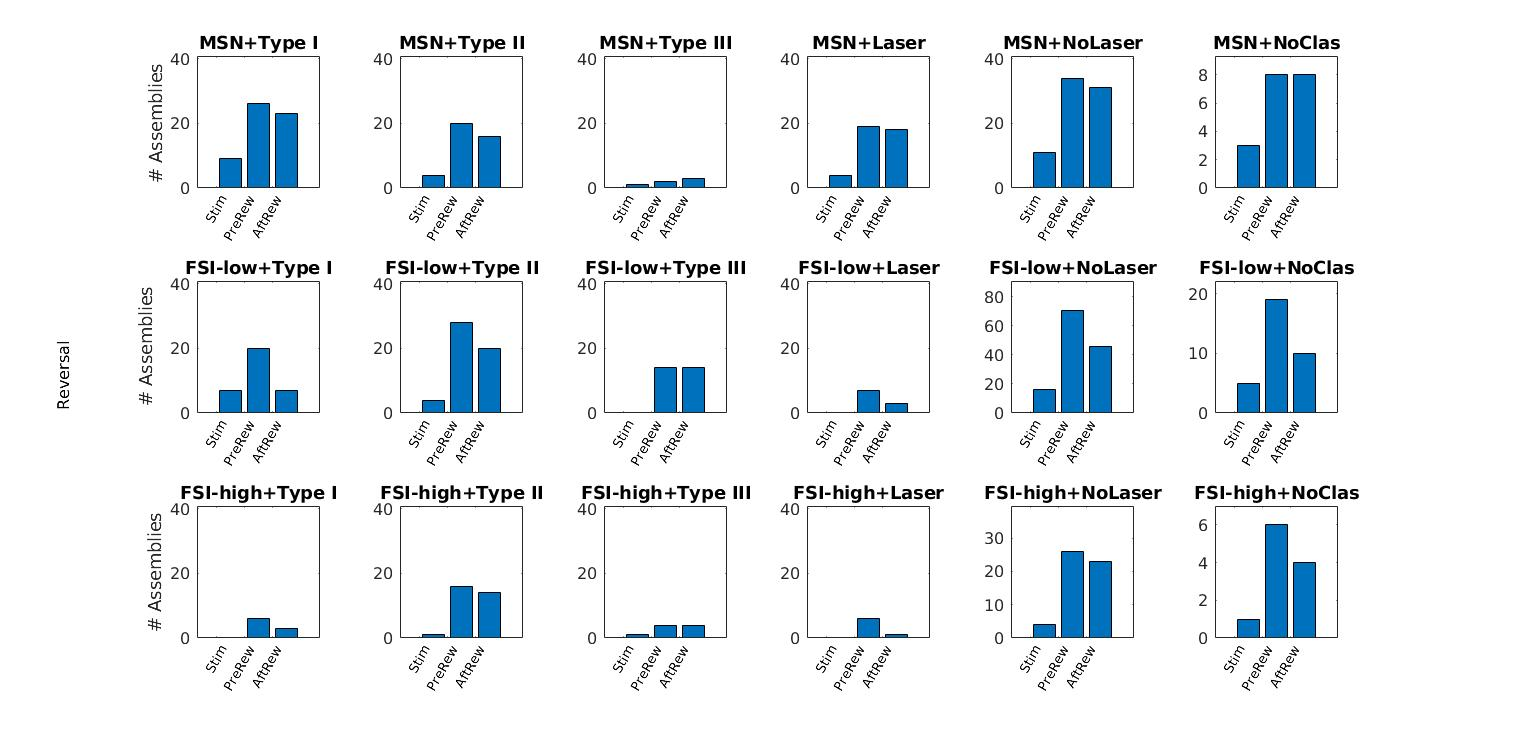
\includegraphics[scale=0.3]{figures/Reversal_Hit_N.jpg}
     \caption{{\color{red}TO MODIFY!!!! BUT THIS IS THE PLOT}}
     \label{fig:histo_taskrel}
 \end{figure}
\begin{figure}
    \centering
    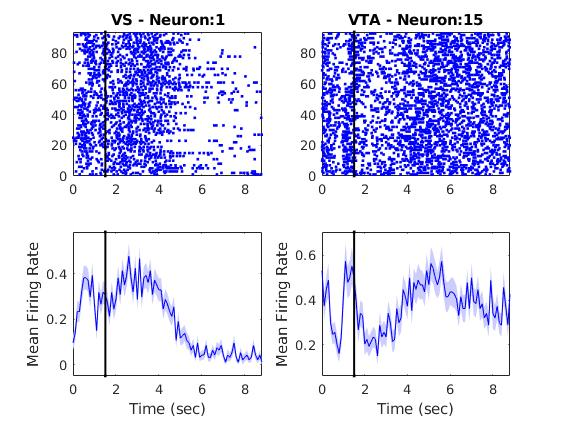
\includegraphics[scale=0.6]{figures/SingleNeus1_15Lastrev1Pru_An_4.jpg}
    \caption{Shift in time of neuronal activity of two units in assembly. }
    \label{fig:NeusInAsse}
\end{figure}

%\section{Discussion}
%\section{Combination of single neuron and assemblies analysis}
%\subsection{Directionality using classification}
\subsection{Significant task related response for typology}
Our interest was focused again to the smallest temporal scale.
Here, the assemblies were pruned according their significant task related activity, that was tested with Friedman's test and a non parametric version of the repeated measures Anova. We preferred to use non-parametric tests to be free from the assumption of gaussianity of the observations. Results of the two tests were consistent each other. The two relevant events of the task were the odor onset and the reward delivery, then we choose whether the assemblies showed a significant activity in three windows: Post-Stimulus [0s, 0.5s], Pre-Reward [-0.5s, 0s], Post-Reward [0s, 05s], the baseline was chosen in the interval [-1s, -0.5s] from the odor onset. Post-hoc analysis were performed using the Bonferroni's criterion {\color{red}check whether the criterion was Bonferroni of some other}. Almost $80\%$ of the VS-VTA assemblies showed a task related activity significant different from the baseline or from another of the windows considered. Of the significant assemblies $\%$ were composed by MSN-Type I units, $\%$ by FSI low-Type I, $\%$ by FSI high-Type I, $\%$ MSN-Type II, $\%$ by FSI low-Type II, $\%$ by FSI high-Type II, the other possible units combinations constitutes a minority and all toghether were the $\%$ {\color{red} Insert numbers of percentage}.

\section{Conclusion}
